\chapter{A Review on 3GPP 5G Security Aspects}

\begin{center}
{\large\uppercase{Rajavelsamy R}} 

\vskip -6pt

Samsung R\&D Institute India – Bangalore (SRI-B)

\bigskip
{\large\uppercase{Debabrata Das}} 

\vskip -6pt

International Institute of Information Technology – Bangalore (IIITB)
\end{center}

\noindent\makebox[\textwidth]{
\includegraphics[width=1.05\paperwidth,height=16cm]{src/Figures/3GPP.jpg}}

\newpage

\begin{multicols}{2}

\section*{Abstract}

5G promises to support new level of use cases that will deliver a better user experience. The 3rd Generation Partnership Project (3GPP) \cite{art4-key01} defined 5G system introduced fundamental changes on top of its former cellular systems in several design areas, including security. Unlike in the legacy systems, the 5G architecture design considers Home control enhancements for roaming customer, tight collaboration with the 3rd Party Application servers, Unified Authentication framework to accommodate various category of devices and services, enhanced user privacy, and secured the new service based core network architecture. Further, 3GPP is investigating the enhancements to the 5G security aspects to support longer security key lengths, False Base station detection and wireless backhaul in the Phase-2 of 5G standardization \cite{art4-key02}. This paper provides the key enhancements specified by the 3GPP for 5G system, particularly the differences to the 4G system and the rationale behind the decisions.

\section{Introduction}

The 3rd Generation Partnership Project (3GPP) is the international standards organization responsible for industry-wide 5G standards \cite{art4-key01}. The security group in 3GPP (Service and System Aspects WG\#3 (SA3)) \cite{art4-key02}, is responsible to specify the security aspects of the cellular systems specified in 3GPP. The 3GPP develops the technical specifications (TS), publishes the TSs under the system ‘Releases’. Each 3GPP Release provides a set of stable features and its functionalities, for the implementation of features at a given point and then permit for the addition of new functionality in the subsequent Releases. The latest Release-15 (Rel-15), published in Dec-2018, specified the first set of TSs for 5G system. As the Release-15 work (often referred as ‘5G Phase 1’) has matured and drawn to 100\% completion, the working groups in 3GPP are focusing now on Release-16 (referred as ‘5G Phase 2’) on the enhancements, which is planned to be published in first quarter of 2020, as shown in Figure~\ref{chap4-fig01}, which is published by the 3GPP\cite{art4-key01}.

This paper provides an outline of the background to the evolution to 5G security aspects and the track the industry/3GPP forum is convincing to realise the benefits that will arise from the deployment of 5G cellular system. The security mechanism in 5G systems has evolved right from the original analog systems through Global System for Mobile Communications (GSM), Universal Mobile Telecommunications System (UMTS) and LTE. The 3GPP \cite{art4-key01} has standardized 5G security mechanisms for authentication and authorization of the subscription, protection (integrity protection and/or encryption) of Access Stratum (AS) signalling messages, Non-Access Stratum (NAS) signalling messages, user data traffic and inter/intra operator network interconnect in its specification TS 33.501\cite{art4-key03}.
\end{multicols}

\setcounter{figure}{0}
\begin{figure}[H]
\centering
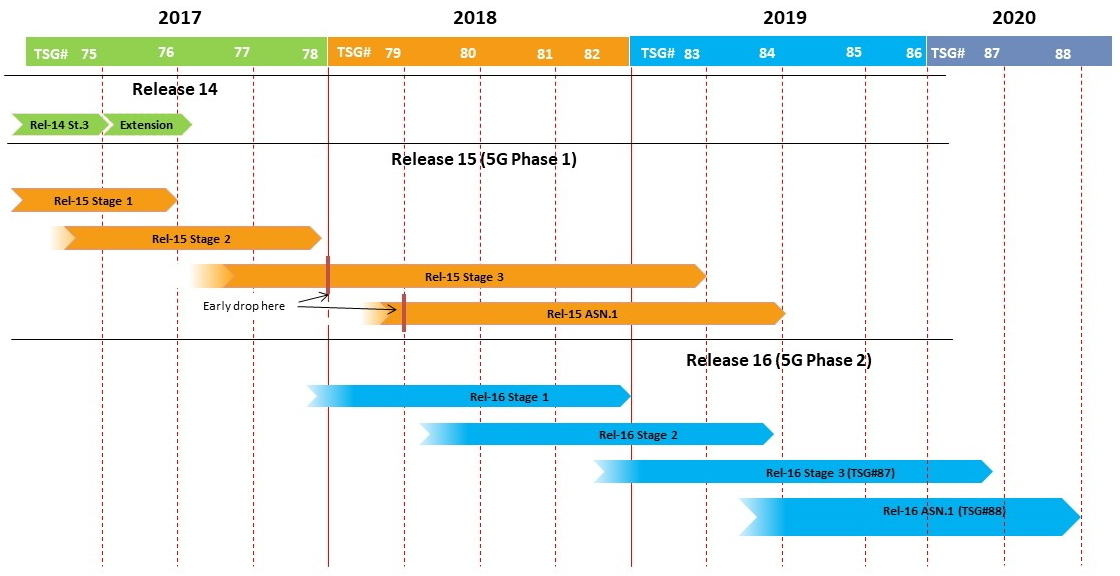
\includegraphics[scale=1.92]{src/Figures/chap4/chap4-fig01.jpg}
\caption{3GPP 5G Release schedule\cite{art4-key01}}\label{chap4-fig01}
\end{figure}

\begin{multicols}{2}

\section{Home Control Enhancements}

\noindent
{\bf {\textit{A. Home Participation in Authentication procedure}}}

Currently, establishment of roaming agreements are based on the trust relationship between the roaming partners. Some operators may wish to decrease the amount of blind trust they have on the roaming partners, as the visited operators, e.g. providing wrong location information of the inbound roamers, for claiming manipulated charging information, may abuse the trust. Thus, the home network operator needs to determine that the subscriber’s location update requested by the roaming partner to the home network has really been authenticated through the visited network, which claims it. In addition, the visited network should not deceive the confirmation message from the User Equipment (UE) with a reasonable probability. Therefore, in 5G system, the AKA method is enhanced to provide an authentication confirmation from the UE via the visited network to the home network. With a direct endorsement from the UE, the home network confirms that the authentication is successful. To obtain such endorsement of the UE’s presence in visited network, the home expects an endorsement parameter \textit{XRES} from the UE via the visited network, similarly the visited network also expects a response from the UE to verify the authenticity of the UE. So when the UE provides the response \textit{RES}, the visited network computes the \textit{HRES} and once it matches, then the response \textit{(RES)} obtained from the UE is further provided to the home network, so that home network checks whether \textit{RES} is same as \textit{XRES}. If it is same, then the UE presence is endorsed and the home network honours the location update from the visited network. 
\begin{figure}[H]
\centering
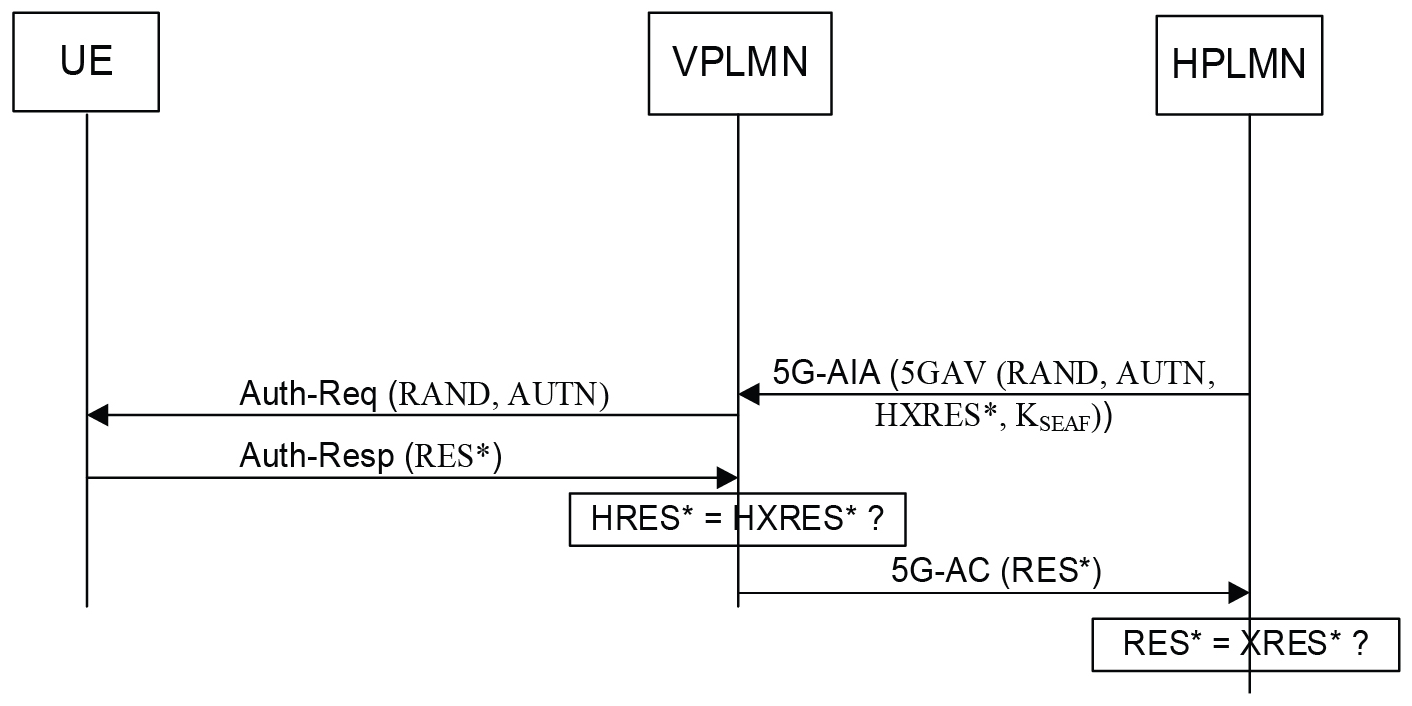
\includegraphics[scale=3]{src/Figures/chap4/chap4-fig02.jpg}
\caption{ Enhanced Authentication Mechanism for more Home Network Control}\label{chap4-fig02}
\end{figure}

\noindent
{\bf {\textit{B. Secure connection between the UE and the Home Network}}}

Unlike the early systems, the 5G system supports end-to-end security between the home network and the UE, for security provisioning of the configuration parameters, using the control plane. Until 5G, the provision of the home network parameters are done as proprietary mechanism (Over-the-Air mechanisms) and there is dependency on the $\text{3}^{rd}$ parties (e.g. Operation and Management servers). The 3GPP enhanced the key hierarchy of the 4G for the 5G and introduced a new key $K_{AUSF}$, derived by the AUSF and the UE, after successful authentication for e2e protection, as shown in Figure~\ref{chap4-fig03} \cite{art4-key03}. By this enhanced key hierarchy, the home network can securely provision the home network configuration parameters like, preferred PLMN list, Routing ID, like so, when the UE is in roaming.
\begin{figure}[H]
\centering
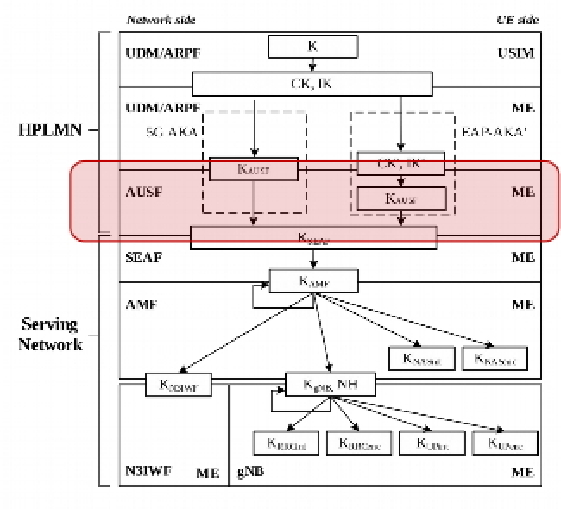
\includegraphics[scale=1.8]{src/Figures/chap4/chap4-fig03.jpg}
\caption{ Enhanced Key hierarchy to support e2e protection between the Home network and the UE}\label{chap4-fig03}
\end{figure}

\noindent
{\bf {\textit{C. Steering of Roaming}}}

The Steering of Roaming is to enable the home network operator to steer its roaming customers (outbound roamers) to its preferred roaming partner (VPLMN) networks to enhance roaming customers’ user experience and to reduce roaming charges. Till 4G (LTE networks), home network is capable to steer its outbound roamers to its preferred VPLMN based either on selective rejection of signaling messages (for e.g., location update procedures) from the VPLMN for the UE or based on proprietary mechanisms (e.g. Over The Air (OTA) commands over SMS or IP to the USIM in the UE). However, the existing mechanisms until in the LTE are not acceptable. It is always possible for the VPLMN to block or corrupt the SMS or IP packet to the UE and the UE is not aware that there is an updated list from the home network. Even if the list over the SMS/IP is received by the USIM, the list will be effective only when PLMN (re)selection is performed by the UE (normally UE in connected state will not perform PLMN (re)selection), until then the non-preferred VPLMN serves the UE. Based on these limitations (which provides unethical commercial benefits for the malicious roaming partners), 3GPP decided the need to define a standardized way to allow a home network to provide its roaming UEs with information about preferred networks and RAT depending on the UE current location. Thus, for 5G system, a new optional (optional for the home network) native support for a secure Steering of Roaming (SoR) solution, using control plane is specified, as shown in Figure~\ref{chap4-fig04}. The objective is that, based on the protected mandatory list of preferred networks and RATs provided by the home network during registration procedure (before transmission and/or reception of the User Plane traffic), the UE may decide to de-register from the current VPLMN and search for a more preferred VPLMN. Since, the home network protects the list using a shared secret Key $K_{AUSF}$ between the UE and the home network, the UE will be able to detect if the VPLMN modified or remove the information and act accordingly.
\begin{figure}[H]
\centering
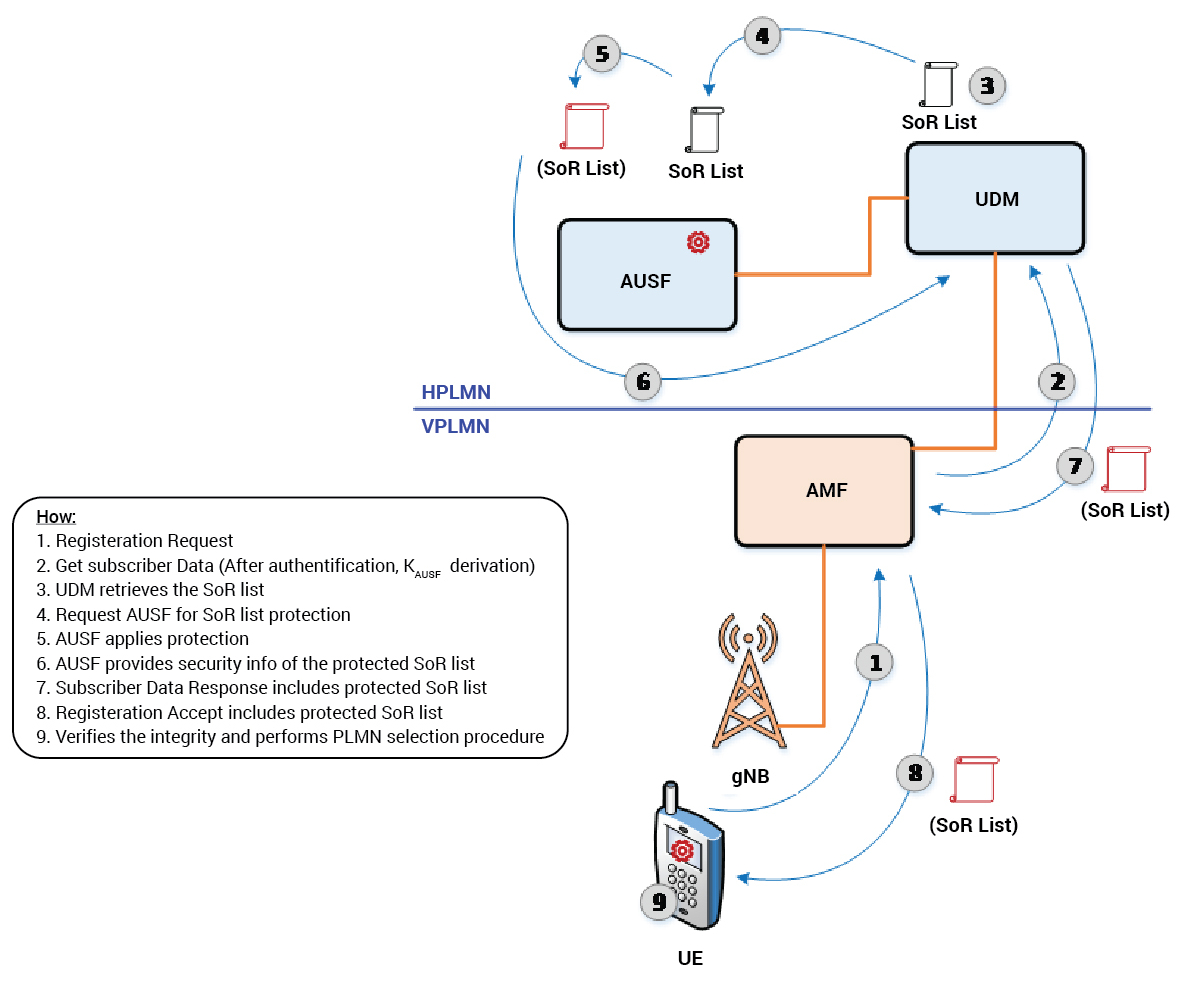
\includegraphics[scale=0.75]{src/Figures/chap4/chap4-fig04.jpg}
\caption{Security mechanism for SoR}\label{chap4-fig04}
\end{figure}

\section{Unified Authentication Framework}

3GPP adopts the most reliable IETF EAP framework for the 5G System, as to support various types of authentication methods and at the same time to support access network agnostic authentication procedure \cite{art4-key03}. Support for various authentication methods is required to support various category of devices that has different secure storage and execution environments. For example, it is efficient and effective to have certificate based authentication for Machine Type communication devices for accessing the Non-public networks, password/biometric based authentication for accessing private network and AKA credentials based authentication for accessing the public networks. Further access agnostic authentication framework is required to access the 5G core network, as to have single authentication framework to support access from multiple access network technologies 5G, WLAN, Wired line access, like so. The EAP framework is used between the UE and network, over the N1 interface to perform network access authentication using the AKA authentication method, either via Next Radio (NR) or via WLAN, as shown in Figure~\ref{chap4-fig05}.
\begin{figure}[H]
\centering
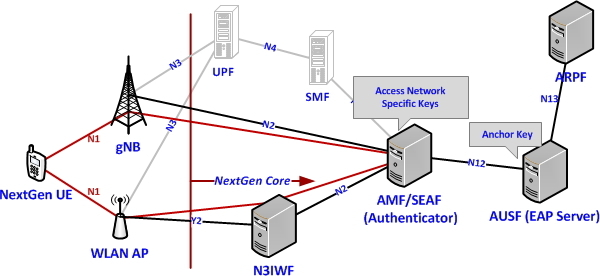
\includegraphics[scale=1.65]{src/Figures/chap4/chap4-fig05.jpg}
\caption{Unified network access authentication framework}\label{chap4-fig05}

\vskip -.4cm
\end{figure}


\section{User Privacy}

\noindent
{\bf {\textit{A. SUPI concealment}}}

\begin{figure}[H]
\centering
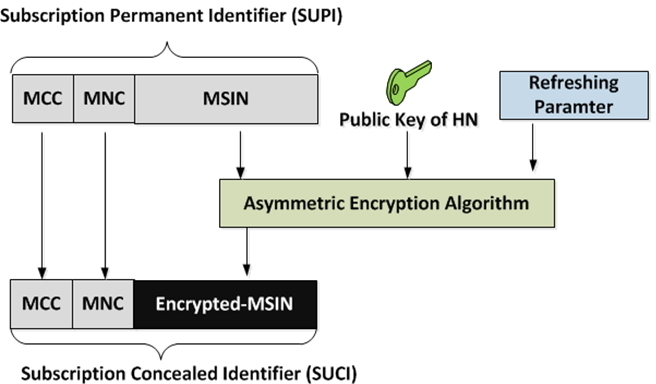
\includegraphics[scale=1.45]{src/Figures/chap4/chap4-fig06.jpg}
\caption{Method of SUPI concealment}\label{chap4-fig06}
\end{figure}

\vskip -.3cm

In 5G system, a globally unique Subscriber Permanent Identifier (SUPI) is allotted for every subscriber. In order to avoid the threats identified till in the 4G system on the IMSI, 3GPP decided not to disclose the SUPI over the air in clear, if decided by the home network (since SUPI is allotted and provisioned by the home operator). The 5G permanent  subscriber identifier SUPI, contains subscriber unique identity  as well as subscription’s home network information (for routing purposes). Therefore, if permanent identifier (subscriber unique identity) is exposed over the air interface in clear (without encryption), then an attack can breach the privacy of the subscriber (track the subscriber and identify the presence of the subscriber) and mount targeted attacks like DoS attack on a particular user. Thus for 5G system, it is recommended not to transmit the permanent identifier in clear. To provide privacy for the subscriber, the 5G specification specified that the UE generates and transmits the Subscription Concealed Identifier (SUCI1), as shown in Figure~\ref{chap4-fig06} using the public key of the home network that was securely provisioned/pre-configured in UE \cite{art4-key03}. Therefore, the SUPI is always transmitted in a concealed form over the air interface. The home network performs the de-concealing of the subscriber unique identity and provides to the serving network.



\noindent
{\bf {\textit{B. Initial NAS protection}}}

A UE initiates registration procedure to register to a PLMN by sending a Registration Request message. The Registration Request message contains sensitive user information(s) e.g. a service user is going to access (e.g. Slice information/identity). The ciphering of NAS message is an optional feature (but highly recommended to enable ciphering) and is based on local regulatory requirement. If a local regulatory requirement mandate to send NAS message ciphered then all the operators in that region should perform encrypted communication over the air. Similarly, if a local regulation mandats not to do ciphering, then the operator will use NULL ciphering procedure i.e. performing ciphering using NULL ciphering algorithm (NEA0), which will result in clear text. If the operator policy is to protect the NAS messages, then 3GPP decided that all sensitive information carried in the NAS messages (even in the initial message) need to be protected. To achieve this requirement, if the 5G Non Access Stratum (NAS) context exists then the UE shall send an Initial NAS message ciphered in a NAS message container of the initial NAS message using the ciphering algorithm of 5G NAS security context \cite{art4-key03}.

Initial NAS message protection mechanism has been introduced to provide the encryption of the sensitive data. In this procedure when the UE does not have 5G NAS security context then the UE will send the sensitive data encrypted after the 5G NAS security context has been established using the NAS ciphering algorithm of the 5G NAS security context. If the UE has a valid NAS security context then the UE encrypts the sensitive data using the NAS ciphering algorithm of the current 5G NAS security context. The NAS ciphering algorithm is chosen as per the local regulation.

\section{Network Security}

\noindent
{\bf {\textit{A. User Plane Security}}}

In legacy systems (2G and 3G), the user plane protection at radio bearer level (Layer 2) protects all the communication between the User Equipment (UE) and the mobile network. It is because most of the services were operator provided services. However, considering Mobile Broadband (MBB) services provided by LTE and beyond wireless networks, it is questionable whether that these systems need to provide radio layer security for all the user plane traffic. Security mechanism at the radio layer should not be a constraint for the emerging Radio Access Network (RAN) technologies in the future, as security procedures are one of the sources of power consumption and also introduce latency.

Thus in 5G System, it is agreed that the use of User Plane protection (Integrity Protection and/or encryption) depends on operator-dependent policy, which means optional for the network to enable the User Plane protection for a PDU session, as shown in Figure~\ref{chap4-fig07}, based on the security policy decided by the operator. The serving network (which may be a roaming partner) can override the security policy of the home network. The operator sets the policy to disable/enable the UP protection for some reason (service-dependent policy, e.g. disabled for online Gaming, enabled for IoT services, etc.).  If bearer level protection is enabled, then all user plane data of a PDU session is encrypted and/or integrity protected based on security policy irrespective of whether the data is already protected or not at the higher layer.
\begin{figure}[H]
\centering
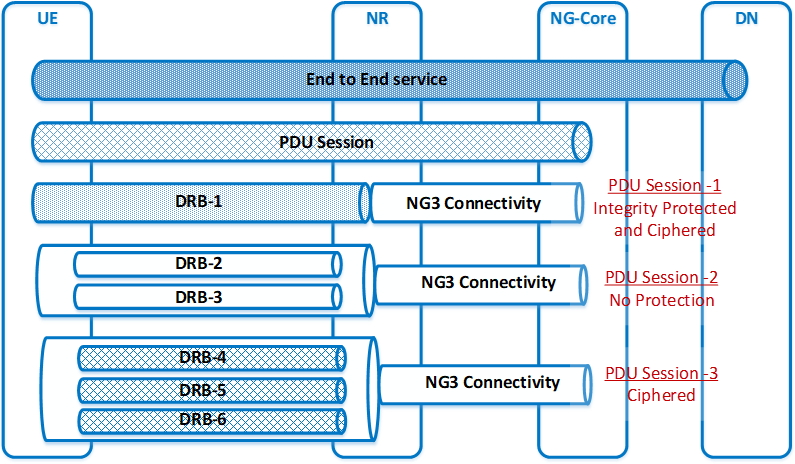
\includegraphics[scale=1.15]{src/Figures/chap4/chap4-fig07.jpg}
\caption{Selective User Plane protection}\label{chap4-fig07}
\end{figure}

\vskip -.3cm

\noindent
{\bf {\textit{B. Service Based Interface security}}}

3GPP is specified to use TLS and Client/Server certificate based authentication for secure communication between the network functions within a PLMN \cite{art4-key03}. 

For inter-PLMN connection, as there are significant number of possible attacks reported on the subscriber’s key theft, when exchanged between the roaming partners, attacks on SS7 like re-routing, attacks on DIAMETER protocol like IP address spoofing, 3GPP decides to specify solution to mitigate the attacks on internetwork interconnect. Therefore, in 5G system, the inter-operator connection is protected using a new network functionality called SEcurity Protection Proxy (SEPP), as shown in Figure~\ref{chap4-fig08}. The SEPP at the edge of the network is used for the protection of the control plane messages between the operator’s networks. The SEPP receives the service layer messages from the network entities and protects them before sending it out of the network (on the N32 interface) and vice versa, that is it receives the messages on the N32 interface (from other networks) and provides to the appropriate network entities after verifying the security.  The SEPP provides both e2e protection and also hop-by-hop protection, as e2e protection is needed for some IEs in the signalling messaged between the NFs across the two PLMNs and e2e protection is provided at the application layer. Also some IEs needs hop-by-hop protection between the adjacent network entities (if there are Internet Protocol (IP) Packet eXchange (IPX) networks) and network layer security or transport layer security is used for hop-by-hop protection.
\begin{figure}[H]
\centering
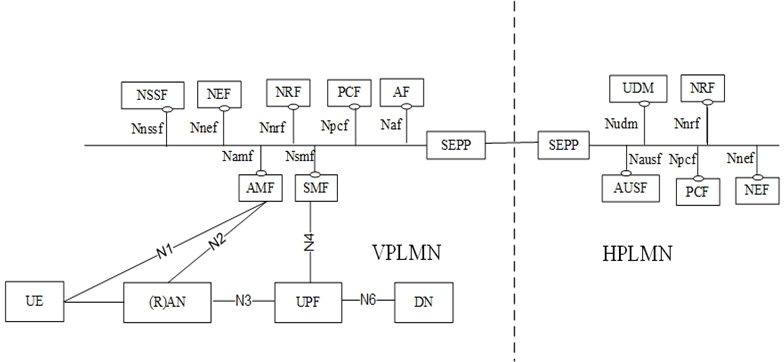
\includegraphics[scale=1.35]{src/Figures/chap4/chap4-fig08.jpg}
\caption{Inter-PLMN Interconnect Protection}\label{chap4-fig08}
\end{figure}

\noindent
{\bf {\textit{C. Northbound APIs}}}

A common API framework within 3GPP is considered, which will allow for a consistent development of northbound APIs i.e. when defining northbound APIs to abstract or expose the underlying 3GPP network capabilities to 3rd party applications \cite{art4-key10}. The common API  aspects considered are onboarding, publishing, discovery, authentication, registration, authorization, logging, charging, monitoring, configuration, topology hiding, and as well as multiple deployment models e.g. centralized vs. distributed, single vs multiple service/API providers. The 3GPP specified specification TS 33.501\cite{art4-key03}, includes the possibility for the 5G system, to support CAPIF. The security aspect of CAPIF is also considered and specified in TS 33.122 \cite{art4-key04}. To secure and authenticate the onboarding of the API invoker to the CAPIF core function (CCF), the API invoker and the CCF establish a TLS session. 

For authentication of the CAPIF-1e reference point, mutual authentication based on client and server certificates is performed between the CCF and the API invoker, using TLS. Further, TLS is used to provide integrity protection, replay protection and confidentiality protection for CAPIF-1e interface. The API invoker and the CCF negotiate a security method over the CAPIF-1e interface that is used by the API invoker and the API exposing function for CAPIF-2e interface authentication and protection. After successful mutual authentication on CAPIF-1e interface, based on the API invoker's subscribed service APIs, access scenarios and AEF capabilities. The CCF chooses the security method and sends the chosen security methods along with the information required for authentication of the API invoker at the AEF to the API invoker. The information may include the validity time of the CAPIF-2e credentials. Based on the selected security method by the CCF, one of the following methods: using TLS-PSK, using PKI, TLS with OAuth token is used by the API invoker and the API exposing function for CAPIF-2e interface authentication and protection, as shown in Figure~\ref{chap4-fig09}.
\begin{figure}[H]
\centering
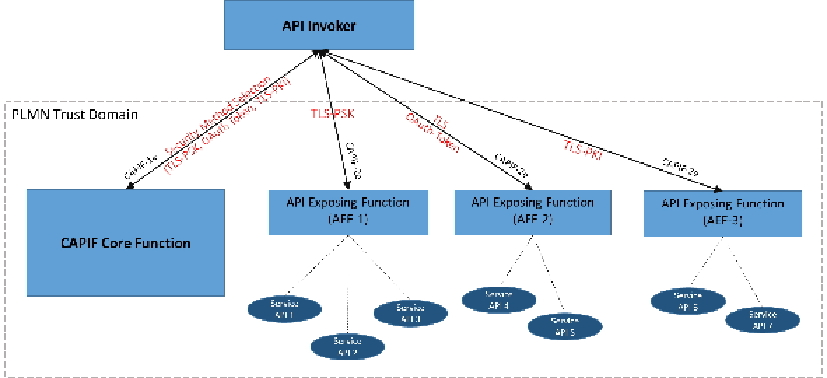
\includegraphics[scale=1.3]{src/Figures/chap4/chap4-fig09.jpg}
\caption{Security Aspects of Common API Framework (CAPIF)}\label{chap4-fig09}
\end{figure}

\section{Upcoming Security Aspects\hfill\break (5G Phase-2)}

\noindent
{\bf {\textit{A. Support for 256-bits keys}}}

It is possible that, quantum computing \cite{art4-key05} will poses a long-term threat to 5G systems. 3GPP decided that threats introduced by the quantum computing requires study in 3GPP, so as to safeguard that 5G systems remain secure also in the future. The 3GPP initiated a study, which focused on the implications of introducing 256-bit cryptographic keys and algorithms (symmetric cryptographic algorithms). Based on the study, it is concluded that there is no immediate need to transition to 256-bit key lengths \cite{art4-key06}, at least in Rel-16. However, the recommendation is that the 5G system may be required to support 256-bit algorithms in future releases.

\noindent
{\bf {\textit{B. IAB Security}}}

3GPP decided to support wireless backhaul/relays in NR  \cite{art4-key07}. To enable faster 5G network deployment scenarios, the support for wireless backhaul and relay links is required, as wireless links enables flexible and dense deployment of NR cells without the need for densification of the transport network proportionately. Amongst several architectures considered for the Integrated Access Backaul (IAB), the majority of companies and operators in 3GPP preferred to follow the CU/DU architecture  \cite{art4-key07}, in which the integrated access backhaul (IAB) node host the DU and MT functionalities and would effectively look like a DU connected through the wireless interface to the controlling CU. As a consequence, the wireless interface between the IAB node and the IAB donor (F1*) is similar to the F1 interface connecting CU and DU. F1* interface will have to exchange packets over the wireless interface, as opposed to the conventional F1 interface, in which F1 packets are exchanged over the wired network. Exchanging packets over the wireless interface create new potential security risks for the IAB deployments. Thus, 3GPP decided to study the security aspects of the IAB architecture (as shown in Figure~\ref{chap4-fig09}) and the protection of the associated wireless backhaul links \cite{art4-key08}. As of writing this paper, 3GPP \cite{art4-key02} is considering use of IPsec for the protection of the wireless F1* interface.
\begin{figure}[H]
\centering
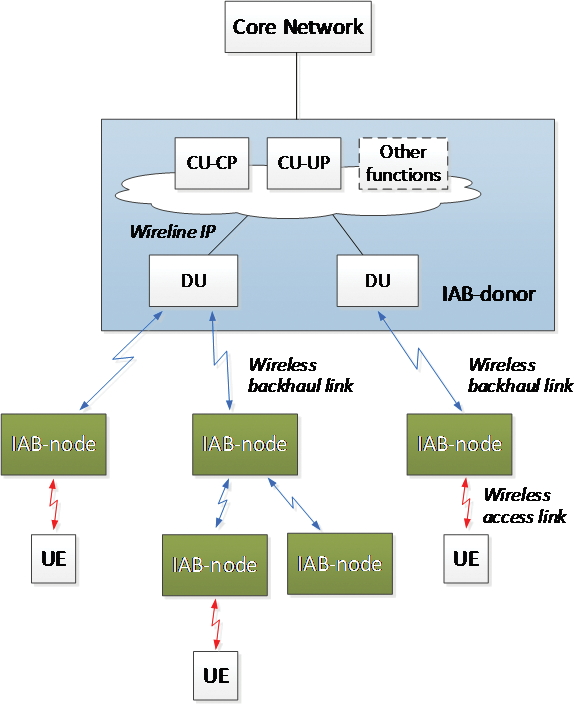
\includegraphics[scale=2.65]{src/Figures/chap4/chap4-fig10.jpg}
\caption{IAB Architecture}\label{chap4-fig10}
\end{figure}

\vskip -.3cm

\noindent
{\bf {\textit{C. False Base Station}}}

In the LTE and also in 5G system, UE obtains some services in the RRC IDLE and RRC INACTIVE state. In the RRC IDLE or in RRC INACTIVE state, UE acquires the system information from the camped cell and uses them to receive paging and obtain other services such as receiving information about the radio configuration for MBMS, D2D, etc. When the UE selects a cell in RRC idle mode, it does not validate whether the cell is authentic or fake cell. As a result, UE may camp on a rogue cell leading to denial of services, as the UE will be missing the following: public safety warnings, mobile terminated services like incoming calls, real-time application (server push services), proximity services, etc. So far the mobile communication system has been focused on providing AS secure communication in the RRC CONNECTED state and security aspects in RRC IDLE state are not considered. As some services are offered to the UE in the RRC IDLE mode through System Information Blocks, it is necessary to consider and ensure the security of the messages carrying the service/service information, even when the UE is in RRC IDLE mode for the next generation systems. Therefore, 3GPP is considering a mechanism (active mechanism), where the UE will verify the authenticity of the cell before camping on it\cite{art4-key09}. 

As of writing this paper, 3GPP \cite{art4-key02} is considered asymmetric cryptography to address the issue of identifying the false base-station. In order to enable the UE to validate the authenticity of received system information, the NR digitally signs the broadcasted system information as shown in Figure~\ref{chap4-fig10}. System information to be broadcasted, Private security key (K-${\text{SIG}}_{Private}$) and Time Counter are input to security algorithm to generate the Digital Signature (DS). The generated DS together with some least significant bits of Time Counter is added to the system information before transmitting over the air. K-$\text{SIG}_{Private}$ is specific to the Tracking area. The private key (K-$\text{SIG}_{Private}$) is provisioned in the NR by the MNO. The public K-$\text{SIG}_{Public}$ key is provisioned by the core network to the UE, when performing location update procedure. Time Counter is maintained based on UTC time.  
\begin{figure}[H]
\centering
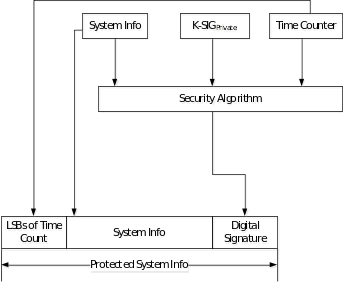
\includegraphics[scale=2.65]{src/Figures/chap4/chap4-fig11.jpg}
\caption{Securing the SI for verification of the authenticity of the NR cell}\label{chap4-fig11}
\end{figure}

On receiving the system information the UE generates digital signature.  The system information with digital signature received, public security key (K-$\text{SIG}_{Public}$) and Time Counter of the time slot in which system information is received are used to check the authenticity of the SI. If authenticity verification is successful, then the system information is authentic and the UE considers the cell as authentic.

The size of the digital signature leads to increase in the signalling overhead. System information is periodically broadcasted, in order to reduce the overhead; protection can be applied once every ‘N’ period instead of every period. However, there are other potential open issues are under consideration, like the UE checks that the timestamp is within an acceptable time-window before it verifies the signature to prevent replay attacks. But, UE does not have access to that accurate clock information for signature verification.

\section{Conclusion}

It is expected from the 5G system to deliver QoS, QoE, reliability and security, at par with previous generation, unlicensed radio access technologies and also with the advancing fixed networking. With the phase-1 specified security mechanism, the 5G system will rule out the vulnerability identified in the legacy wireless generations and the foreseen security threats. 3GPP will drive the work on the Phase-2 topics further to standardize the new enhancements, if any.\raisebox{-.1cm}{
\includegraphics[scale=.9]{src/Figures/circledC.eps}}

\begin{thebibliography}{99}
\bibitem{art4-key01} \url{http://www.3gpp.org/}
\bibitem{art4-key02} \url{https://www.3gpp.org/Specifications-groups/sa-plenary/54-sa3-security}
\bibitem{art4-key03} 3GPP TS 33.501: “Security architecture and procedures for 5G System”
\bibitem{art4-key04} 3GPP  TS 33.122: “Security aspects of Common API Framework (CAPIF) for 3GPP northbound APIs”.
\bibitem{art4-key05} Sandor Imre , Ferenc Balazs, Quantum Computing and Communications: An Engineering Approach, John Wiley \& Sons, 2005.
\bibitem{art4-key06} TR 33.841: “Study on the support of 256-bit algorithms for 5G”.
\bibitem{art4-key07} TS 38.401: “NG-RAN; Architecture description”.
\bibitem{art4-key08} TR 33.824: “Study on security aspects of Integrated Access and Backhaul (IAB) for Next Radio (NR)”.
\bibitem{art4-key09} TR 33.809: “Study on 5G security enhancements against false base stations”.
\bibitem{art4-key10} TS 23.222: “Common API Framework for 3GPP Northbound APIs”.
\end{thebibliography}
\end{multicols}


\noindent
\begin{tabular}{V{2.5}cp{14cm}V{2.5}}
\clineB{1-2}{2.5}
 &\\
\raisebox{-4.4cm}{
\includegraphics[scale=4]{src/Figures/authors/Rajavelsamy.png}} & 

\centerline{\large\bf Rajavelsamy R}

\bigskip
Rajavelsamy R is an Architect (General Manager) in the Standards Team of Samsung R\&D Institute India, Bangalore. He received Bachelor of Engineering Degree in Electronics and Communication Engineering and Master of Technology Degree in Computer Science and Engineering. He joined Samsung Electronics, at its India office in 2003 and has been with its Standards Team, focusing on research and standardization of wireless mobile communications. He has 15+ years of rich experience in Security system architectures, Security protocols, Wireless cellular communications systems and protocols, where he has contributed in research and standardization of Samsung Telecommunication products. Since 2004, he has been actively involved in contributing and participating in 3GPP SA3 meetings representing Samsung. He has actively contributed since Rel-6, e.g. WCDMA, IWLAN, H(e)NB, LTE, MTC, ProSe, MCX, CAPIF, 5G standardization. He also served as Vice Chairman of 3GPP SA3 WG (July 2007 to Nov 2009). He is active as rapporteur for several 3GPP SA3 work items specifically, MTC, CAPIF, IAB, SCAS-UPF.\\
&\\  
\raisebox{-5cm}{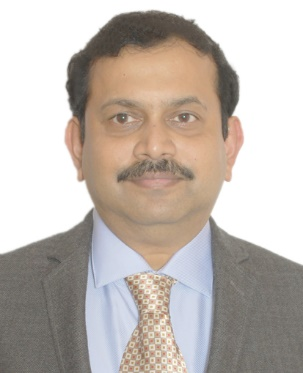
\includegraphics[scale=.33]{src/Figures/authors/D-Das.png}} & 

\centerline{\large\bf Dr. Debabrata Das}

\bigskip
Dr. Debabrata Das is Professor at IIIT-Bangalore (IIIT-B). Before joining IIIT-B, he had served at G S Sanyal School of Telecommunication at IIT Kharagpur and later at Kirana Networks in New Jersey, USA. At present, he is Principal Investigator (PI) of projects from Department of Electronics and Information Technology, Government of India on Green Broadband Wireless Network and Nokia Research on IoT. He was PI of sponsored projects from Intel, Hewlett Packard, Microsoft, Motorola Research, Nokia, Govt. of India on areas of IMS and Broadband Wireless MAC/QoS/Energy-saving, TVWS and Security. He has more than 125 peer reviewed papers in different journals and International conferences. He has 1 accepted US patent and 10 more are under review. Dr. Das received his Ph.D. degree from IIT-Kharagpur and MTech from IIT-Varanasi. He is Board Member of IIIT-Bhubaneswar; Technical and Empower Committee member of e-Governance, Govt. of Karnataka; He is Fellow of Institution of Electronics \& Telecommunication Engineers (IETE) and Fellow-IE. Dr. Das is recipient of Global IEEE MGA Achievement Award 2012 and Prof. K Sreenivasan memorial outstanding teaching award in the areas of Electronics and Telecommunication in 2017.\\
&\\
\clineB{1-2}{2.5}
\end{tabular}
